\section{Generating Functions}

Generating functions are functions that encode sequences of numbers as the coefficients of power series. One example are the moment generating functions in probability theory, though they are generally extremely useful in combinatorics problems and, almost equivalently, discrete probability problems. 

\citeasnoun{bogart2004combinatorics} approaches the concept in terms of \textit{Picture Functions}. For each element $s\in S$, there is a picture function $P(s)$, so that, for example, the multiset $\{1,1,2\}$ can be written as $P(1)^1 P(2)$. Collections of combinations can be rewritten in terms of sums and products, which enables factorization and overall easier accounting. Combinations with particular properties can be filtered by looking at exponents. 

The picture function enables writing down combinations of elements as an enumerating function $E_P(s)$. For example, the enumerating function for all multisets that include either one or two times some element $a$ and between zero and two times some element $b$ is written:

\begin{equation}
\begin{array}{rl}
E_P(s) &= P(a)+ P(a)^2 + P(a)P(b) + P(a)^2P(b) +  + P(a)P(b)^2 + P(a)^2P(b)^2\\
&\left(P(a) + P(a)^2\right)\left(1 + P(b) + P(b)^2\right)
\end{array}
\end{equation}



\subsection{Example: Binomial Coefficients}

Consider the case of a collection of $n$ indistinguishable objects $s$, and write $P(s) = x$. Then the enumerator for selecting any subset of those $n$ objects is given by: 

\begin{equation}
E_P(s) = \prod_i^n (x^0+x^1) = (1+x)^n = \sum_i^n {n \choose i}x^i
\end{equation}

Where each term $(x^0 + x^1)$ corresponds to the two options of either excluding a particular element ($x^0$) or including a particular element ($x^1$). The exponent of the expanded product encodes how many objects were included into a particular subset. This is one way of "proving" the binomial coefficients, and one can says $(1_x)^n$ is the generating function for the binomial coefficients ${n \choose i}$. 


\subsection{Example: Basket of Goods}

An apple costs $20c$, a pear costs $25c$ and a banana costs $30c$. How many different fruit baskets can be bought for $100c$?

By replacing the picture function $P(s)$ with $x$, it was possible to identify subsets of $n$ objects by looking at the exponent of $x^n$ in the enumerating function. In this case, the exponent is supposed to show the price. This can be done by writing $P(apple) = x^{20}, P(pear) = x^{25}$ and $P(banana) = x^{30}$. 

\begin{equation}
E_P(s) = \left( \sum_{i=0}^5 x^{20} \right)\left( \sum_{i=0}^4 x^{25} \right)\left( \sum_{i=0}^3 x^{30} \right)
\end{equation}

Which results in some power series of the form:

\begin{equation}
E_P(s) = 1x^0 + 1x^{20} + 1x^{25} + 1x^{30} + 1x^{40} +... + 2x^{60} + ... + 1x^{290}
\end{equation}

To obtain the number of combinations that correspond to a cost of exactly $100c$, one can apply the operator $\frac{1}{n!}\frac{d^n}{dx^n}$ and set $x=0$ to obtain the desired term. This is what is done with moment generating functions in statistics. 

But actually it is easier to think through what the coefficients will be so that:

\begin{equation}
\sum_{l=0}^{n+m+h}d_l x^l = \left(\sum_{i=0}^n a_i x^i\right)\left(\sum_{j=0}^m b_j x^j\right)\left(\sum_{k=0}^h c_k x^k\right)
\end{equation}

\begin{equation}
d_l = \sum_{\begin{array}{c}i,j,k\\i+j+k=l\end{array}} a_i b_j c_k
\end{equation}

If the coefficients are all '1', which is the case for these combinations, then:

\begin{equation}
d_l = \sum_{\begin{array}{c}i,j,k\\i+j+k=l\end{array}} 1 = {l + 3 - 1 \choose l}
\end{equation}

Which is the number of all multisets of size $l$ and 3 classes. In this case the coefficients are equal to 1 for i=20, j=25, and k=30, and zero otherwise, so that there are 4 ways of summing to 100. Hence, $d_{100} = 4$ for the basket of goods above.

The sum can also be rewritten:

\begin{equation}
d_l = \sum^l_{i=0}\sum^{l-i}_{j=0} a_i b_j c_{l-i-j}
\end{equation}


Of course, this is the discrete version of a convolution. So, it is no surprise that the addition of random variables winds up being a convolution.


\subsection{Example: Dice}

How many ways are there for $n$ dice with $k$ faces to show $s$ eyes?

\begin{equation}
E_P = \left(\sum_{i=0}^\infty a_i x^i\right)^n = \sum_{i=0}^{\infty}d_i x^i
\end{equation}

Where $a_i = 1\ \forall i\in(1,k)$ and $a_i = 0$ otherwise.

\begin{equation}
E_P = \left(\sum_{i=1}^k x^i\right)^n = \left(x(1-x^k)\sum_{i=0}^\infty x^i\right)^n = x^n\left(\frac{1-x^k}{1-x}\right)^n = x^n \left(\sum_{i=0}^n (-1)^i {n \choose i} x^{ik}\right)\left(\sum_{j=0}^{\infty} (-1)^j {-n \choose j} x^j\right)
\end{equation}

The coefficient for $x^s$ is given the sum:

\begin{equation}
d_s = \sum_{ki+j=s-n} (-1)^{i+j}{n \choose i}{-n \choose j}\\
i \in [0,n] \\
j \in [0,\infty]
\end{equation}

Where the indices $i$ and $j$ satisfy $ki+j = s-n$. For example, for $s=7$, $n=2$ and $k=6$:

\begin{equation}
6i+j = 7-2 = 5s
\end{equation}

Holds for $i=0, j=5$:

\begin{equation}
d_s = (-1)^5 {2 \choose 0}{-2 \choose 5} = (-1)^{10} 1 {2+5-1 \choose 5} = {6 \choose 5} = \frac{6!}{5!1!} = 6
\label{eq:d6}
\end{equation}

Indeed, there are 6 ways for two d6 to add to 7:

\begin{equation}
[6,1],[5,2],[4,3],[3,4],[2,5],[1,6]
\end{equation}


\begin{figure}
\centering
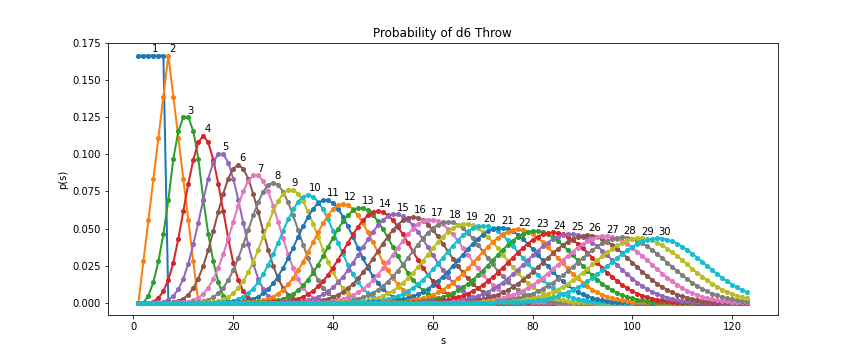
\includegraphics[scale=0.5]{d6throw.png}
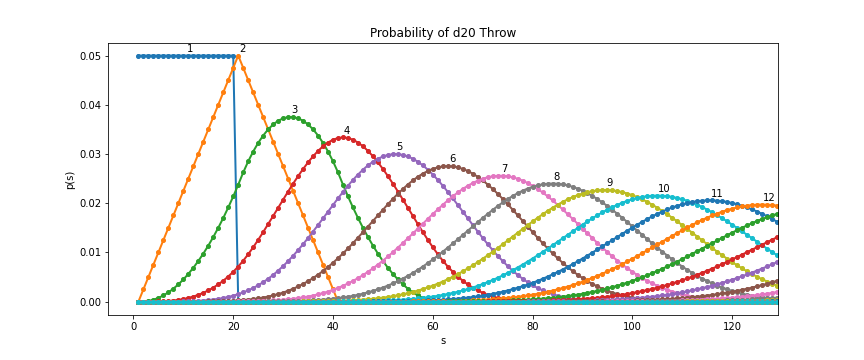
\includegraphics[scale=0.5]{d20throw.png}
\caption{Probability of the sum of 6-sided and 20-sided dice, calculated with Eqn. \ref{eq:d6}. Note that these are simply the convolutions of $n=1,2,3,...$ square waves, which rapidly adopts the shape of a Bell curve.}
\end{figure}
